\documentclass[conference]{IEEEtran}
\usepackage{newtxtext,newtxmath}
\usepackage{graphicx}
\usepackage{amsmath}
\usepackage{booktabs}
\usepackage{url}
\usepackage[hidelinks]{hyperref}
\usepackage{xcolor}

\title{Wrist Force-Torque Input and Arm Compliance in Learned 1\,mm-Clearance Insertion: Behavior Cloning, ACT and Diffusion Policy in Simulation}

\author{\IEEEauthorblockN{Pavan Yadav Annappa}
\IEEEauthorblockA{Friedrich-Alexander-Universit\"at Erlangen-N\"urnberg, Germany\\
(M.Sc. student; independent work)\\
pavanyadava07@gmail.com}}

% abstract heading without the class's long dash
\makeatletter
\def\abstract{\normalfont\bfseries\@IEEEabskeysecsize\noindent\textit{\abstractname:}\ \relax}
\def\endabstract{\relax\par\vspace{0.5\baselineskip}}
\makeatother

\begin{document}
\maketitle

\begin{abstract}
We study learned insertion of a 6\,$\times$\,10\,$\times$\,4\,cm part into a fixture with 1\,mm clearance per side on a simulated Franka Panda with a wrist force-torque (F/T) sensor. Three learners are trained on the same 479 scripted demonstrations and evaluated on the same 200 unseen scene seeds, under nominal perception and with the fixture position perceived 2\,mm off. The policies receive no camera input: they observe the robot state, simulated noisy part and fixture poses, and the filtered wrist wrench. A three-layer MLP trained by behavior cloning succeeds in 179/200 nominal episodes and 84/200 with the 2\,mm error. Removing the F/T input lowers these to 156/200 and 47/200 (paired exact McNemar $p = 1.4\times10^{-3}$ and $2.9\times10^{-5}$); most of the added failures never reach 5\,N of contact force. With LeRobot implementations and the settings reported here, Diffusion Policy reaches 75/200 and ACT 9/200 on the same data. Replacing position control with a torque-level Cartesian impedance controller raises the scripted expert from 165/200 to 194/200 under the 2\,mm error ($p = 1.1\times10^{-6}$) at a lower median peak contact force (26.8 vs.\ 45.8\,N), but behavior cloning of that compliant expert reaches only 51/200. All results are from simulation, and the negative results are reported as measured.
\end{abstract}

\section{Introduction}
Tight-clearance insertion is a common step in industrial assembly: the approach and grasp are easy, while the last millimetres decide whether a part is seated. Small errors in the perceived fixture pose put the part on a wall edge or a chamfer, and the controller then has to recover through contact. Imitation learning methods such as Action Chunking with Transformers (ACT)~\cite{zhao2023act} and Diffusion Policy~\cite{chi2023diffusion} have been shown on fine manipulation, and open libraries such as LeRobot~\cite{cadene2024lerobot} make them easy to apply to a new task. It is less clear how they compare with a plain behavior-cloning (BC) baseline~\cite{pomerleau1988alvinn} on a small, low-dimensional contact task, how much the wrist F/T signal contributes, and how the low-level controller under the policy changes the outcome.

This paper reports a controlled simulation study of these questions on one task. The contributions are:
\begin{itemize}
\item An insertion task in MuJoCo~\cite{todorov2012mujoco} on the Franka Panda model from MuJoCo Menagerie~\cite{zakka2022menagerie}: 1\,mm clearance per side, a 2\,mm lead-in chamfer, a wrist F/T sensor, and a controlled 2\,mm perception error on the fixture position.
\item A comparison of an MLP BC policy, ACT and Diffusion Policy trained on the same scripted demonstrations and evaluated on the same 200 unseen seeds, with Wilson intervals~\cite{wilson1927} and paired exact McNemar tests~\cite{mcnemar1947}.
\item An F/T ablation for BC and Diffusion Policy, with a failure-mode breakdown from the logged episodes.
\item A comparison of IK position control with a torque-level Cartesian impedance controller~\cite{hogan1985impedance}, for the scripted expert and for BC.
\item A list of simulation fixes that were needed before the task was meaningful, and the negative results (ACT, BC under impedance control).
\end{itemize}
Code, per-episode results and the scripts that produce every number are public.\footnote{\url{https://github.com/pavanyadava007/assembly-lab}; the mapping from each number in this paper to its source file is in \texttt{paper/NUMBERS.md}.}

\section{Related Work}
\textbf{Imitation learning.} Behavior cloning regresses actions on observations~\cite{pomerleau1988alvinn}; its errors compound once the policy leaves the demonstration distribution~\cite{ross2011dagger}. ACT~\cite{zhao2023act} predicts chunks of future actions with a conditional VAE and a transformer and was shown on fine bimanual tasks. Diffusion Policy~\cite{chi2023diffusion} models the action sequence with a denoising diffusion process and executes it in a receding-horizon manner. Mandlekar et al.~\cite{mandlekar2021matters} showed that design choices and data quality strongly affect offline imitation results. We use the LeRobot~\cite{cadene2024lerobot} implementations of ACT and Diffusion Policy with DDIM sampling~\cite{song2021ddim}.

\textbf{Contact-rich insertion.} Learned peg insertion has used reinforcement learning with force feedback~\cite{inoue2017deep} and self-supervised fusion of vision and touch~\cite{lee2019vision}. Impedance control~\cite{hogan1985impedance} regulates the relation between motion and contact force rather than position alone, which is the usual reason it is preferred for insertion. Here we keep perception fixed and low-dimensional and vary only the learner, the F/T input and the low-level controller.

\section{Task and Simulation Setup}
\begin{figure}[t]
\centering
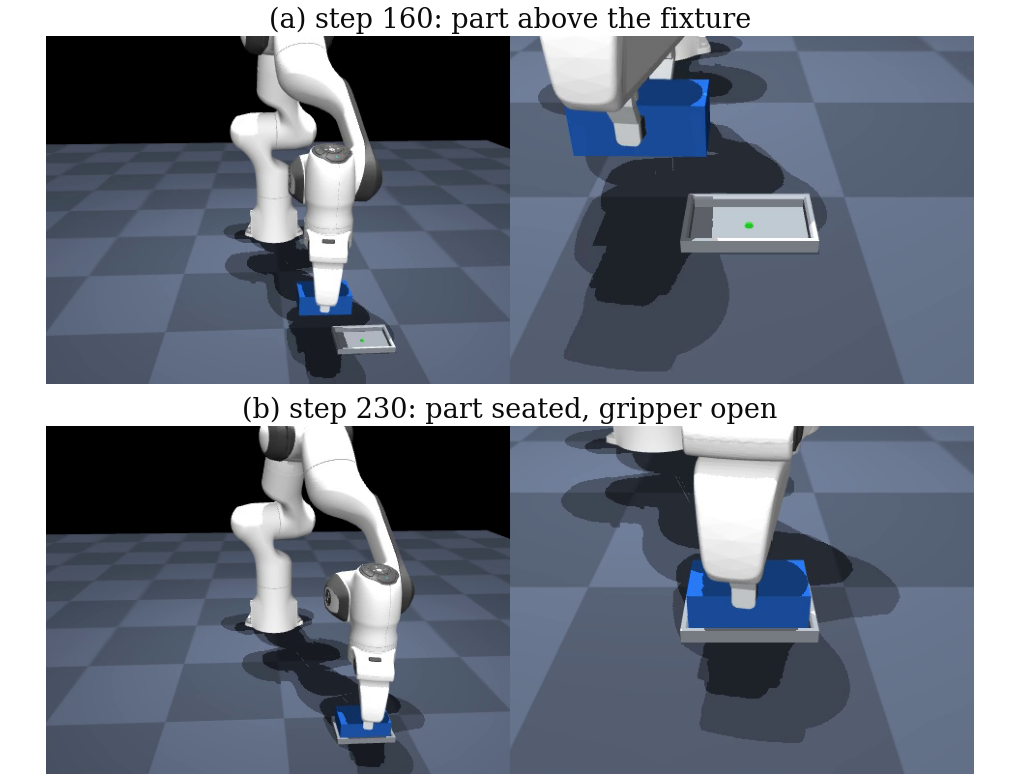
\includegraphics[width=\columnwidth]{fig_scene.png}
\caption{The task in simulation (scripted expert, seed 100003, fixture perceived 2\,mm off; left: front camera, right: close camera). The cameras are used only for these renderings; no policy receives images.}
\label{fig:scene}
\end{figure}
\textbf{Scene.} The Franka Panda model from MuJoCo Menagerie runs in MuJoCo with a 2\,ms physics step. A 0.3\,kg box (6\,$\times$\,10\,$\times$\,4\,cm) starts on the table with its position randomized by $\pm$4\,cm and its yaw by $\pm$0.35\,rad. It has to be placed into a pocket 12\,mm deep whose inner size leaves 1\,mm clearance per side; the inner top edge has a 2\,mm 45-degree chamfer. The fixture position is randomized by $\pm$2\,cm. Fig.~\ref{fig:scene} shows the scene.

\textbf{Sensing and observation.} A 6-axis F/T site is placed between flange and hand. The wrench is bias-corrected at reset, corrupted with 0.3\,N Gaussian noise per control step, and low-pass filtered. The 23-D observation contains the tool position, tool yaw (sine, cosine), gripper width, the perceived part position (0.5\,mm noise), the part yaw relative to the tool (folded for the box's $\pi$ symmetry), the perceived fixture position (0.5\,mm noise), the part position relative to the tool, and the scaled wrist wrench. There is no camera input.

\textbf{Actions and control.} At 20\,Hz the policy outputs a Cartesian tool displacement (up to 1\,cm per step), a yaw increment (up to 0.08\,rad), and a binary gripper command. In the default \emph{position} mode the target is converted to joint position targets by damped least-squares inverse kinematics with a null-space posture term. The commanded point may lead the measured tool point by at most 6\,mm downward (2\,cm overall), so a blocked descent builds bounded force. In the \emph{impedance} mode the arm actuators become torque motors and a Cartesian impedance law $\tau = J^\top(K e - D\dot{x}) + \tau_{\text{bias}} + \tau_{\text{null}}$ runs at 500\,Hz, with $K$ = 800, 800, 1500\,N/m (laterally softer than vertical), 60\,N\,m/rad in rotation, critical damping, gravity and Coriolis compensation, and a null-space posture stiffness of 10. In this mode three more observation dimensions give the commanded point minus the tool point (26-D in total).

\textbf{Perception conditions.} \emph{Nominal}: 0.5\,mm pose noise only. \emph{2\,mm off}: the observed fixture position is shifted by 2\,mm in a random horizontal direction, so the part usually lands on the chamfer or wall and the policy has to recover.

\textbf{Success.} An episode (at most 400 steps, 20\,s) succeeds when the part lies flat in the pocket (bottom within 3\,mm of the floor, centre within 4\,mm in each axis, tilt below the threshold $R_{zz} > 0.995$) \emph{and} the gripper has opened and moved at least 3\,cm above the part. We also log the peak part-fixture contact force and the final horizontal placement error.

\textbf{Scripted expert.} The expert approaches, grasps, lifts, aligns the part over the \emph{perceived} fixture position and then runs one compliant insertion phase: it descends slowly; while the part touches a wall or chamfer it moves away from the contact and adds that shift to its goal; it backs off if the wrist force exceeds 50\,N and lifts to retry when wedged. The expert reads the contact side from the simulator's contact list, which the learned policies cannot do: they only see the wrist wrench.

\textbf{Demonstrations.} 500 episodes with seeds 0 to 499 were recorded; half had a fixture perception error drawn uniformly from 0 to 2.5\,mm. The expert succeeded in 240/240 episodes without and 239/260 with an error. Only the 479 successful episodes were kept (104,848 frames at 20\,Hz); 279 of them contain a force-guided recovery. Demonstrations are scripted, not teleoperated.

\section{Policies and Evaluation}
\textbf{MLP BC.} Three hidden layers of 512 units (GELU), MSE loss on the 5-D action, AdamW (learning rate $3\times10^{-4}$), cosine schedule, 30{,}000 steps with batch 256 (540{,}165 parameters).

\textbf{Diffusion Policy} (LeRobot 0.4.4): 1-D convolutional UNet with channels 128/256/512, 2 observation steps, horizon 16, 8 executed actions per chunk, 100 training timesteps and DDIM with 10 inference steps (16.7\,M parameters).

\textbf{ACT} (LeRobot 0.4.4): chunk size 20 with 10 executed actions, model width 256, 8 heads, 4 encoder layers and 1 decoder layer, CVAE objective with LeRobot's default KL weight of 10, no temporal ensembling (7.4\,M parameters). ACT and Diffusion Policy were trained for 30{,}000 steps with batch 256 and AdamW at learning rate $10^{-4}$. For both, the observation is split into a robot-state vector (tool pose, gripper width and, unless ablated, the 6-D wrench) and an environment-state vector (part and fixture poses). The images that both architectures normally use are not provided.

\textbf{Ablations.} Each of BC and Diffusion Policy is retrained without the wrench input. Diffusion Policy is also evaluated with re-planning every 2 actions instead of 8, and ACT with re-planning every action. A separate BC policy is trained on 497 demonstrations recorded by the expert under impedance control and evaluated under impedance control.

\textbf{Protocol.} Every policy is evaluated on the same 200 seeds starting at 100{,}000, which never overlap the demonstration seeds, in both perception conditions. Success rates carry 95\% Wilson score intervals~\cite{wilson1927}. Because all policies see the same scenes, pairs of policies are compared with the exact two-sided McNemar test~\cite{mcnemar1947} on the discordant episodes. Training ran on one NVIDIA L4 GPU shared with other jobs; evaluation ran on CPU. A single training seed was used per policy. Table~\ref{tab:train} lists model sizes and training cost.

\begin{table}[t]
\centering
\caption{Model size and training cost (30{,}000 steps, batch 256). The GPU was shared with other jobs, so times are indicative only; the BC ablation was trained on CPU while the GPU was occupied.}
\label{tab:train}
\footnotesize
\begin{tabular}{@{}lrrl@{}}
\toprule
Policy & Parameters & Time & Device \\
\midrule
MLP BC & 540{,}165 & 0.7\,min & NVIDIA L4 \\
MLP BC, no F/T & 537{,}093 & 17.0\,min & CPU \\
ACT & 7{,}415{,}621 & 33.6\,min & NVIDIA L4 \\
Diffusion Policy & 16{,}651{,}653 & 29.8\,min & NVIDIA L4 \\
Diffusion Policy, no F/T & 16{,}565{,}637 & 25.2\,min & NVIDIA L4 \\
\bottomrule
\end{tabular}
\end{table}

\section{Results}
\begin{table}[t]
\centering
\caption{Insertion success on 200 unseen seeds (95\% Wilson interval in \%). Error and force are medians in the nominal condition (error over successful episodes, force over all episodes).}
\label{tab:main}
\setlength{\tabcolsep}{3pt}
\footnotesize
\begin{tabular}{@{}lcccc@{}}
\toprule
Policy & Nominal & 2\,mm off & Err. & Force \\
\midrule
Expert, position & 200 (98-100) & 165 (77-87) & 0.63\,mm & 30.7\,N \\
Expert, impedance & 200 (98-100) & 194 (94-99) & 1.02\,mm & 22.1\,N \\
\midrule
MLP BC & 179 (84-93) & 84 (35-49) & 0.62\,mm & 30.5\,N \\
MLP BC, no F/T & 156 (72-83) & 47 (18-30) & 0.76\,mm & 24.2\,N \\
MLP BC, impedance & 51 (20-32) & 38 (14-25) & 0.78\,mm & 23.6\,N \\
\midrule
Diffusion Policy & 75 (31-44) & 63 (25-38) & 0.82\,mm & 51.2\,N \\
DP, re-plan every 2 & 75 (31-44) & 59 (24-36) & 0.94\,mm & 47.5\,N \\
DP, no F/T & 55 (22-34) & 52 (20-32) & 0.85\,mm & 51.7\,N \\
\midrule
ACT & 9 (2-8) & 8 (2-8) & 0.58\,mm & 74.6\,N \\
ACT, re-plan every 1 & 10 (3-9) & 9 (2-8) & 0.39\,mm & 63.5\,N \\
\bottomrule
\end{tabular}
\end{table}

\begin{figure}[t]
\centering
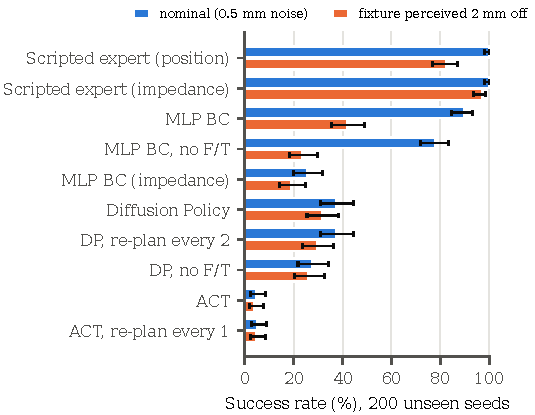
\includegraphics[width=\columnwidth]{fig_success.pdf}
\caption{Success rates of all policies in both perception conditions (same data as Table~\ref{tab:main}).}
\label{fig:success}
\end{figure}

Table~\ref{tab:main} and Fig.~\ref{fig:success} summarize all runs.

\textbf{Learner comparison.} The MLP BC policy is the strongest learner: 179/200 (89.5\%) nominal with a median final placement error of 0.62\,mm, and 84/200 with the 2\,mm error. Diffusion Policy reaches 75/200 and 63/200. On the same seeds BC succeeds where Diffusion Policy fails in 112 nominal episodes and the reverse happens in 8 ($p = 1.4\times10^{-24}$); with the 2\,mm error the split is 61 vs.\ 40 ($p = 0.046$). Re-planning Diffusion Policy every 2 instead of 8 actions leaves the nominal count at 75/200; the two variants disagree on 88 seeds, 44 in each direction, so the shorter open-loop horizon changes which episodes succeed but not how many. With 479 demonstrations and a 23-D state, the larger generative models did not outperform the MLP under the settings used here; we did not tune them further.

\textbf{ACT (negative result).} ACT with the settings above succeeds in only 9/200 nominal episodes, and 10/200 when re-planning after every action. It is not failing to reach the fixture: 163 of its 191 nominal failures exceed 5\,N of contact force. The final horizontal error of the failed episodes has a median of 20.4\,mm (quartiles 6.7 and 39.9\,mm), and the median peak contact force is 74.6\,N, compared with 30.5\,N for BC. We did not diagnose this further; possible causes include the learning rate (ten times LeRobot's ACT preset), the KL weight, and the absence of image features the architecture was designed around.

\textbf{Force-torque ablation.} Table~\ref{tab:ft} lists the paired comparisons. For BC, removing the wrench lowers success from 179 to 156 nominal ($p = 1.4\times10^{-3}$) and from 84 to 47 with the 2\,mm error ($p = 2.9\times10^{-5}$). For Diffusion Policy the drop is significant in the nominal condition (75 to 55, $p = 0.012$) but not with the 2\,mm error (63 to 52, $p = 0.23$).

\begin{table}[t]
\centering
\caption{Paired F/T ablation on the same 200 seeds (exact McNemar). ``Only F/T'': episodes that succeed only with the wrench input; ``Only no F/T'': the reverse.}
\label{tab:ft}
\footnotesize
\begin{tabular}{@{}llccc@{}}
\toprule
Policy & Condition & Only F/T & Only no F/T & $p$ \\
\midrule
MLP BC & nominal & 36 & 13 & $1.4\times10^{-3}$ \\
MLP BC & 2\,mm off & 57 & 20 & $2.9\times10^{-5}$ \\
Diffusion Policy & nominal & 39 & 19 & $1.2\times10^{-2}$ \\
Diffusion Policy & 2\,mm off & 40 & 29 & $2.3\times10^{-1}$ \\
\bottomrule
\end{tabular}
\end{table}

\begin{figure}[t]
\centering
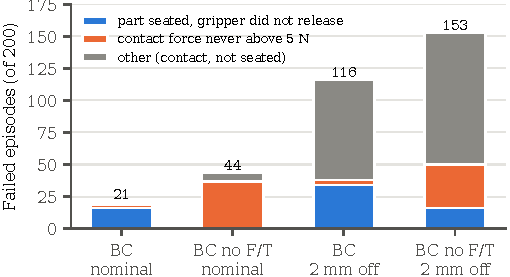
\includegraphics[width=\columnwidth]{fig_failures.pdf}
\caption{Failure modes of MLP BC with and without the wrist wrench, from the per-episode logs. ``Seated'' means the part was in the pocket at some step but the success condition (release and retreat) was not met.}
\label{fig:failures}
\end{figure}

\textbf{Failure modes.} Fig.~\ref{fig:failures} splits the BC failures by the logged episode data. Without the wrench, 37 of the 44 nominal failures never exceed 5\,N of part-fixture contact force: the part does not reach the fixture with any appreciable force (in the recorded videos the policy hovers above the pocket), which is consistent with it having no signal that contact has or has not happened. With the wrench, the main remaining nominal failure is different: in 16 of 21 failed episodes the part was seated but the gripper did not open and retreat. Under the 2\,mm error most failures of both variants are contact without seating (78 of 116 with F/T, 103 of 153 without).

\textbf{Position vs.\ impedance control.} Under nominal perception the scripted expert succeeds in all 200 episodes with either controller; under position control the part touches a wall or the chamfer during insertion in 95 of them, and in all 200 episodes with the 2\,mm error. The 35 position-control failures under the 2\,mm error end either in the align phase (17) or in the insertion phase (17), i.e.\ the expert keeps re-aligning or stays wedged until the time limit; one ends during the final retreat. Under the 2\,mm error impedance control raises it from 165/200 to 194/200 (33 episodes succeed only with impedance, 4 only with position control; $p = 1.1\times10^{-6}$), and the median peak contact force falls from 45.8 to 26.8\,N (Fig.~\ref{fig:force}). We attribute this to the lower lateral stiffness: the chamfer can push the part sideways into the pocket instead of the arm holding it against the edge. Learning does not transfer this gain in our setup. BC trained on 497 impedance-mode demonstrations and run under impedance control reaches only 51/200 nominal and 38/200 with the 2\,mm error, even with the commanded-point offset added to the observation. The compliant arm lags its command, so the expert's action depends on controller state that a single-step policy captures poorly. This is an open problem in this study.

\begin{figure}[t]
\centering
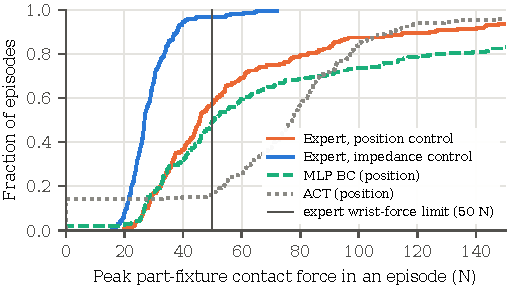
\includegraphics[width=\columnwidth]{fig_force.pdf}
\caption{Distribution of the peak part-fixture contact force per episode with the 2\,mm perception error (200 episodes each).}
\label{fig:force}
\end{figure}

\textbf{Simulation fixes.} Several defects had to be fixed before the task measured what it was meant to. (i) The Menagerie gripper actuator squeezed the 6\,cm part with only about 3\,N, so the 0.3\,kg part slipped out on lift; its gains were raised tenfold, giving about 30\,N. (ii) Grasping 9\,mm above the part centre let the pads catch only the top edge, and the part hung tilted by about 25 degrees; grasping 6\,mm above the centre keeps the tilt below 1.4 degrees while the fingertips still clear the pocket walls. (iii) The first expert recovery (lift and retry in fixed 1.5\,mm steps) overshot, and sliding along the wall in contact oscillated; the single compliant insertion phase with a force limit and a wedge escape described above brought the expert to 200/200 nominal. (iv) Under impedance control the expert initially oscillated when it added the full tool error to its command at every step; it now steers the commanded point plus 0.15 times the tool error. (v) The commanded point is limited to lead the measured tool point by at most 6\,mm downward, an admittance-style limit, so a blocked descent under position control builds bounded force instead of driving the arm through the fixture.

\section{Discussion}
\textbf{Why the small model did best here.} The MLP acts at every 20\,Hz step on the current wrench, while ACT and Diffusion Policy execute parts of predicted chunks. Chunked execution alone does not explain the gap: Diffusion Policy re-planning every 2 actions had the same success count, and ACT re-planning every action barely changed. The task state is low-dimensional and fully given, so the extra capacity of the generative models may not be needed, while their default settings were designed for image inputs and other data scales. We did not run the tuning that would separate these explanations, so this remains a hypothesis.

\textbf{What the paired evaluation adds.} Because every policy saw the same 200 scenes, the exact McNemar test uses only the episodes on which two policies disagree. For Diffusion Policy with and without the wrench (nominal), the Wilson intervals overlap (31-44\% and 22-34\%), but the paired test still separates them ($p = 0.012$). The paired view also showed that two Diffusion Policy variants with identical success counts (75/200) disagree on 88 of 200 scenes. Reporting only marginal success rates would hide this.

\textbf{The gripper-release failure.} With the wrench input, 16 of the 21 nominal BC failures have the part seated but never released. The gripper command is a thresholded output of a regression head, and the switch from closed to open is a rare, sharp event in the demonstrations. A separate classifier for the gripper or a seating-detection condition would be natural fixes; we have not tested them.

\textbf{Compliance and learning.} The impedance controller helped the scripted expert, but the BC policy trained on its demonstrations failed far more often than the position-control policy (134 seeds succeed only under position control and 6 only under impedance control, nominal). The comparison changes both the demonstrations and the controller, so it does not isolate one cause. A policy that outputs impedance targets with history, or one trained with on-policy corrections~\cite{ross2011dagger}, are candidates.

\section{Limitations}
\begin{itemize}
\item \textbf{Simulation only.} No real robot was used. Contact, friction and the F/T signal come from MuJoCo and were not validated against hardware.
\item \textbf{No vision.} The policies take no camera input. Part and fixture poses are given as state with simulated Gaussian noise and an imposed offset; a real system would have to estimate them from images.
\item \textbf{Scripted demonstrations.} All demonstrations come from a scripted expert that has privileged access to the simulator's contact list. A browser teleoperation tool exists in the repository, but no human demonstrations were recorded or used.
\item \textbf{One task, one seed.} One part geometry, one clearance and one training seed per policy. The demonstrations are filtered to successful episodes.
\item \textbf{Untuned baselines.} ACT and Diffusion Policy were run with LeRobot settings adapted to a state-only input and were not tuned; their numbers indicate what these settings achieve on this task, not the best these methods can do.
\end{itemize}

\section{Conclusion}
On a simulated 1\,mm-clearance insertion with state input, a small MLP trained by behavior cloning outperformed LeRobot's ACT and Diffusion Policy on the same demonstrations and seeds. The wrist F/T input mattered for both BC and Diffusion Policy, most visibly as the signal that tells the policy contact has occurred. A Cartesian impedance controller made the scripted expert recover from a 2\,mm perception error far more often and with lower contact force, but cloning that compliant expert failed. Learning policies that exploit compliance, adding vision, and validating on hardware are the next steps.

\bibliographystyle{IEEEtranH}
\bibliography{refs}

\end{document}
